\section{Le matériel}

\subsection{Intérêt}
\begin{frame}{Pourquoi un autre clavier}
    \begin{itemize}
	\item Les claviers standards héritent des lourdeurs du passé: touches en diagonale, position  du retour à la ligne, du backspace, … \pause
	\item Il existe des claviers ergonomiques, bien plus pratiques (clavier matriciel, …).
    \end{itemize}
\end{frame}

\subsection{Exemples}
\begin{frame}{Exemples — Typematrix}
  \begin{figure}
    \centering
    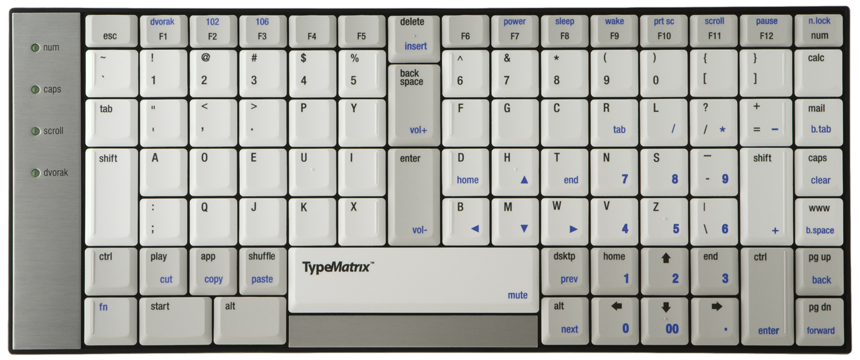
\includegraphics[height=100pt]{images/2030-dvorak.png}
  \end{figure}
\end{frame}

\begin{frame}{Exemples — Truly-Ergonomics}
  \begin{figure}
    \centering
    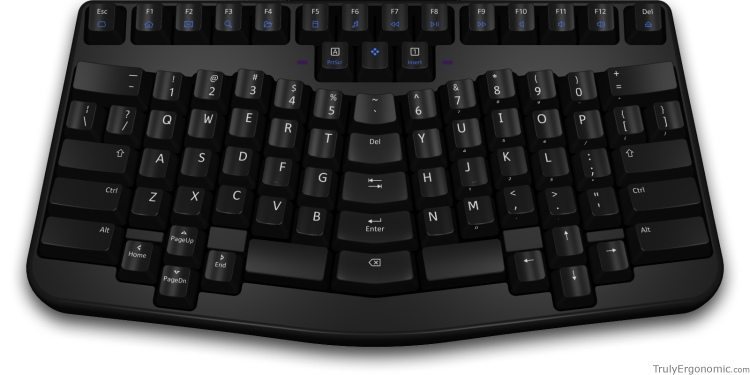
\includegraphics[height=100pt]{images/t_e_keyboard.jpg}
  \end{figure}

  Et d’autres encore~: Kinesys, …
\end{frame}
